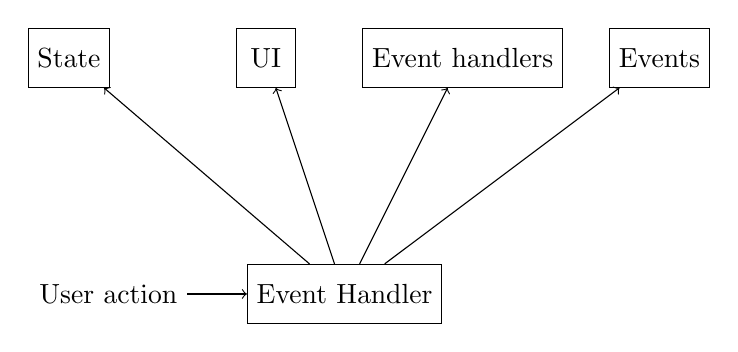
\begin{tikzpicture}
  % Nodes
  \node (state) [rectangle, draw, minimum height=0.75cm, minimum width=1cm] at (-3.5, 0) {State};
  \node (ui) [rectangle, draw, minimum height=0.75cm, minimum width=0.75cm] at (-1, 0) {UI};
  \node (eventH) [rectangle, draw, minimum height=0.75cm, minimum width=0.75cm] at (1.5, 0) {Event handlers};
  \node (event) [rectangle, draw, minimum height=0.75cm, minimum width=0.75cm] at (4, 0) {Events};
  \node (module) [rectangle, draw, minimum height=0.75cm, minimum width=0.75cm] at (0, -3) {Event Handler};
  \node (event0) [] at (-3, -3) {User action};
  % Arrow
  \draw[->] (module) to[] node[midway, above] {} (ui);
  \draw[->] (module) to[] node[midway, above] {} (state);
  \draw[->] (module) to[] node[midway, above] {} (event);
  \draw[->] (module) to[] node[midway, above] {} (eventH);
  \draw[->] (event0) to[] node[midway, above] {} (module);
  %\draw[->] (p) to[out=60, in=120] node[midway, above] {Html/State} (i);
  %\draw[->] (i) to[out=-120, in=-60] node[midway, above] {Msg/State} (p);
  % Header
\end{tikzpicture}
